\section{Results}

\begin{itemize}
    \item Methods on how we're doing simulations and results (with simulations and experimental data)
    \begin{itemize}
        \item Different SNRs and maybe even use CAPs
        \item Selection of HRF explained if both use the same but it's different from what's used for simulating.
        \begin{itemize}
            \item What happens? For example with gamma for simulating.
        \end{itemize}
        \item Selection of regularization parameter
        \begin{itemize}
            \item Present with real data on a voxel
        \end{itemize}
    \end{itemize}
\end{itemize}

With the aim of making a fair comparison of the two methods, we first compared their hemodynamic response functions. Figure~\ref{fig:hrf_diff} shows the difference in the hemodynamic response function that PFM and TA use by default; the SPMG1 and the HRF resulting from the linear differential operator respectively. A clear difference is observable in that the PFM hemodynamic response function begins at zero while the TA HRF starts at 1. Hence, the Total Activation HRF starts close to its peak, which is advanced around 2.5 frames with respect to PFM. Another difference worth mentioning is that PFM normalizes its HRF to a peak amplitude of 1, whereas the TA HRF is not normalized.

\begin{figure}[h]
    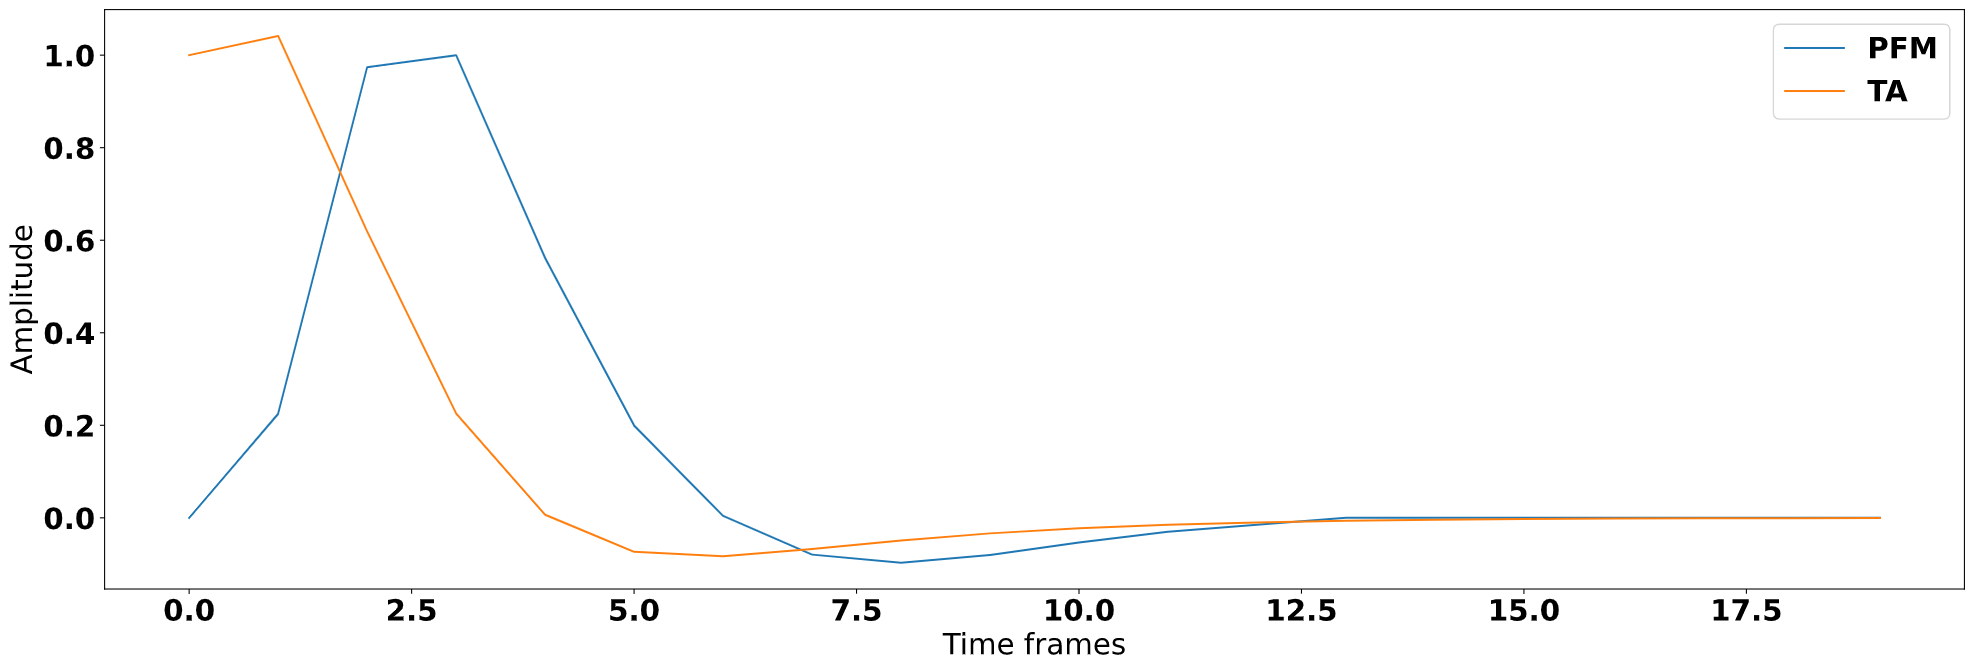
\includegraphics[width=\columnwidth]{figures/hrf_diff.png}
    \caption{Diffence in the HRF of PFM (blue) and TA (orange).}
\label{fig:hrf_diff}
\end{figure}

While Paradigm Free Mapping allows for the use of any hemodynamic response function --- the columns of the design matrix \(\mathbf{H}\) are composed by shifted versions of the HRF --- the linear differential operator in TA is tailored for a fixed HRF. Hence, for practical reasons, we reproduced the HRF in the Total Activation filter and incorporated it into the PFM formulation.

\subsection{Selection of the regularization parameter based on the estimation of the noise}

\subsubsection{Simulated data}

\subsubsection{Experimental data}

\subsection{Selection of the regularization parameter by solving the regularization path}

\subsubsection{Simulated data}

\subsubsection{Experimental data}